\paragraph{Row \& Column counter}
\paragraph{Address counter}
\paragraph{Max \& Min calculator.}

Il modulo Max \& Min calculator permette di trovare i valori massimo e minimo dei pixel presenti nell'immagine.
Il funzionamento del modulo è semplice. Vengono impiegati due registri: MAX e MIN, nei quali alla fine del calcolo saranno presenti rispettivamente il valore massimo e minimo dei pixel dell'immagine.
Inizialmente,(con l'ausilio del segnale "init") viene caricato nei registri MAX e MIN il valore del primo pixel dell'immagine. Successivamente, per ogni altro pixel dell'immagine, lo si confronta con i valori contenuti nel registro MAX e MIN e, se il valore del pixel è maggiore del massimo (contenuto in MAX) o minore del minimo (contenuto in MIN), si aggiornano i valori nei due registri.
Il calcolo termina dopo aver letto e processato l'ultimo pixel dell'immagine.

\begin{figure}[h!] %%%%     H al posto di h! se dà problemi      %%%%%
  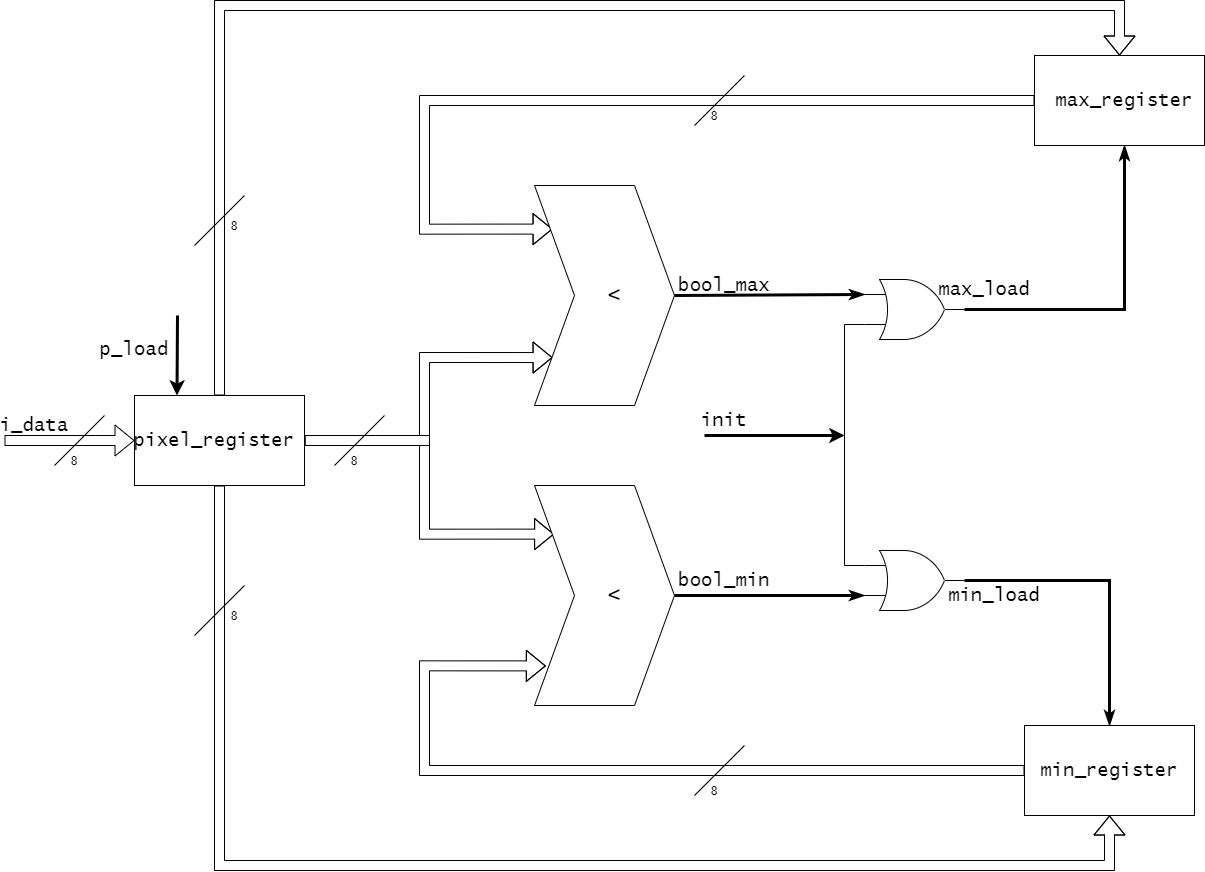
\includegraphics[width=\linewidth]{max_min_module}
  \caption{Max \& Min calculator module.}
  \label{fig:maxMin}
\end{figure}

\paragraph{New pixel value}
